% Unofficial University of Cambridge Poster Template
% https://github.com/andiac/gemini-cam
% a fork of https://github.com/anishathalye/gemini
% also refer to https://github.com/k4rtik/uchicago-poster

\documentclass[final]{beamer}

% ====================
% Packages
% ====================

\usepackage[T1]{fontenc}
\usepackage[size=custom,width=121.92,height=91.44,scale=1.0]{beamerposter}
\usetheme{gemini}
\setbeamerfont{title}{family=\sffamily, series=\bfseries, size=\fontsize{60}{72}}
\usecolortheme{gemini}
\usepackage{graphicx}
\usepackage{booktabs}
\usepackage[numbers]{natbib}
\usepackage{tikz}
\usepackage{pgfplots}
\pgfplotsset{compat=1.14}
\usepackage{anyfontsize}
\usepackage[style=numeric, backend=biber]{biblatex}
\addbibresource{poster.bib} % Or whatever your .bib file is named

% ====================
% Lengths
% ====================

% If you have N columns, choose \sepwidth and \colwidth such that
% (N+1)*\sepwidth + N*\colwidth = \paperwidth
\newlength{\sepwidth}
\newlength{\colwidth}
\setlength{\sepwidth}{0.025\paperwidth}
\setlength{\colwidth}{0.3\paperwidth}

\newcommand{\separatorcolumn}{\begin{column}{\sepwidth}\end{column}}

% ====================
% Title
% ====================

\title{Kinematic Optimization of SHMS and HMS using Hydrogen Elastic Reactions\\for Deuteron Electro-Disintegration Studies at Jef\kern ferson Lab}

\author{\underline{Walker Law}\inst{1}, Pramila Pokhrel\inst{2}, Carlos Yero\inst{2}}

\institute[shortinst]{\inst{1} Coe College, Cedar Rapids, IA \samelineand \inst{2} The Catholic University of America, Washington, D.C.}

% ====================
% Footer (optional)
% ====================

\footercontent{
  \raisebox{.8ex}{\href{mailto:wllaw23@coe.edu}{wllaw23@coe.edu}}
  \hfill
  \hspace{3.25cm}\raisebox{.8ex}{\href{https://github.com/Walker-Law/reu2025}{github.com/walker-law/reu2025}}
  \hfill
  \raisebox{0.8ex}{\href{https://linkedin.com/in/walker-law}{linkedin.com/in/walker-law}}
}

% (can be left out to remove footer)

% ====================
% Logo (optional)
% ====================

% use this to include logos on the left and/or right side of the header:
% \logoright{\includegraphics[height=7cm]{logo1.pdf}}
% \logoleft{\includegraphics[height=7cm]{logo2.pdf}}

% ====================
% Body
% ====================
\begin{document}

% Refer to https://github.com/k4rtik/uchicago-poster
% logo: https://www.cam.ac.uk/brand-resources/about-the-logo/logo-downloads
\addtobeamertemplate{headline}{}
{
\begin{tikzpicture}[remember picture,overlay]

  % Coe logo top left (unchanged)
  \node [anchor=north west, inner sep=3cm] at ([xshift=-2.25cm,yshift=.25cm]current page.north west)
    {
\includegraphics[height=6cm]{logos/CoeLogo.png}}; 
    
    \node [anchor=north west, inner sep=3cm] at ([xshift=9.25cm, yshift=1.5cm]current page.north west){
\includegraphics[height=8cm]{logos/cua logo.png}}; 

  % jlab logo top right (fixed)
  \node [anchor=north east, inner sep=3cm] at ([xshift=3cm,yshift=0cm]current page.north east)
    {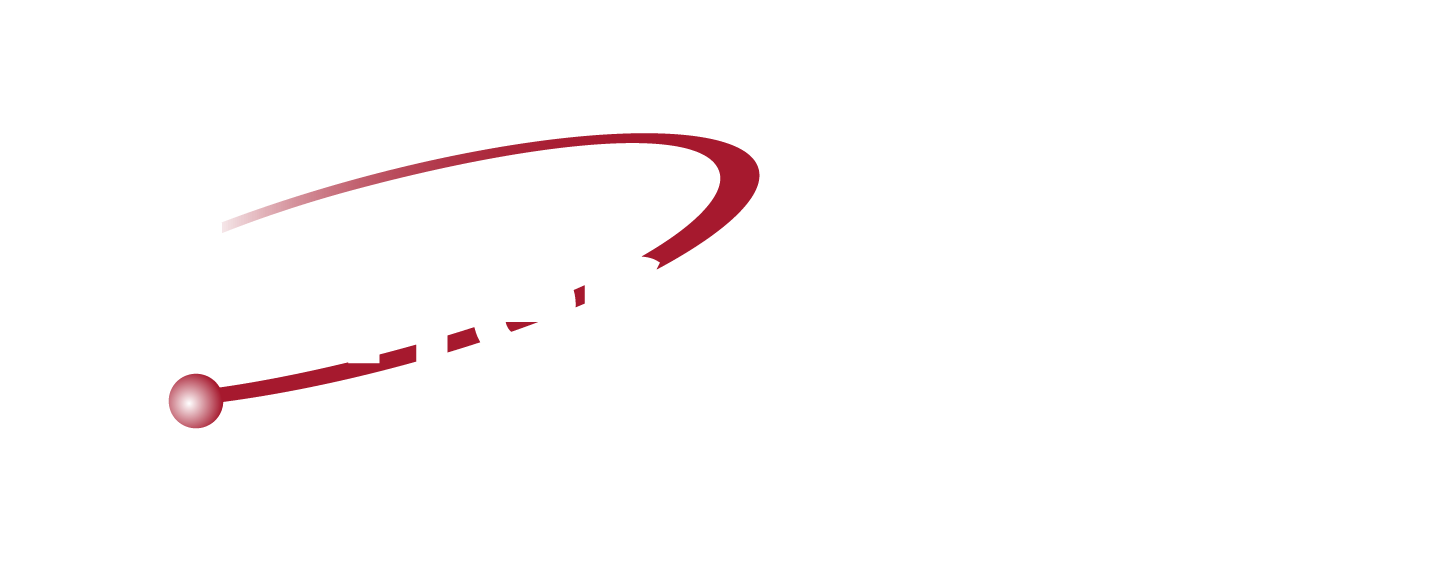
\includegraphics[height=5cm]{logos/Jlab.png}};

    \node [anchor=north east, inner sep=3cm] at ([xshift=-9cm,yshift=2cm]current page.north east)
    {
\includegraphics[height=9cm]{logos/nsflogo.png}};
\end{tikzpicture}

}

\begin{frame}[t]
\begin{columns}[t]
\separatorcolumn

\begin{column}{\colwidth}
\vspace{-.5cm}
  \begin{exampleblock}{Abstract}
    Deuteron electro-disintegration $(D(e,e'p)n)$ is a nuclear reaction in which an electron beam collides with a deuteron nucleus, ejecting the proton and causing the neutron to recoil. The $D(e,e'p)n$ experiment tests various theoretical frameworks, such as Final State Interaction (FSI) and Plane Wave Impulse Approximation (PWIA). To study the $(D(e, e'p)n)$ reaction at Thomas Jefferson National Accelerator Facility (JLab), we optimized the kinematic measurements of the Super High Momentum Spectrometer (SHMS) and High Momentum Spectrometer (HMS) using chi-squared optimization on a hydrogen elastic scattering reaction ($H(e,e')p$) using experiment reconstruction (data) and Monte Carlo simulation (SIMC). The chi-squared optimization method implemented calculates the optimal global spectrometer offsets to best align the SIMC and data histograms. This study prepares the SHMS and HMS for accurate kinematic measurements during future $D(e,e'p)n$ studies at JLab.
    \end{exampleblock}
\vspace{-0.5cm}
  \begin{block}{Kinematic Diagrams}
  \vspace{0cm}
  \begin{figure}
      \centering
      \includegraphics[width=.9\textwidth]{deuteron electrodisint kinematics.png}
      \vspace{-1cm}
      \caption{Diagram of Deuteron Electro-Disintegration Kinematics \cite{yero2020thesis}.}
      \label{fig:deuteron-kinematics}
   \end{figure}
\vspace{-1cm}
\begin{itemize}
   \item An electron beam interacts with the deuteron nucleus, removing the proton from the nucleus via a virtual photon and causing the neutron to recoil.
   \item Neutron momentum and trajectory are reconstructed from the measured proton and electron momenta.
\end{itemize}
      \vspace{-.75cm}
  \begin{figure}
      \begin{tikzpicture}[>=latex,scale=1.45]
        % Incoming electron
        \draw[->, blue, line width=3pt] (-8, 0) node[left] {$e$} node[left, xshift=3cm, yshift=1.5cm]{$E\approx|\vec{k}|$}
        -- (0, 0) 
          node[midway, above] {$\vec{k}$};
        % Outgoing electron
        \draw[->, blue, line width=3pt] (0, 0) -- (8.66025404, 2.5) 
          node[midway, above] {$\vec{k}'$} 
          node[right] {$e'$}
          node[right, above, xshift=-1cm, yshift=.5cm] {$E'\approx|\vec{k'}|$};
        % Projections of k' (blue, dotted)
        \draw[dotted, blue] (8.66025404, 2.5) -- (8.66025404, 0) 
          node[midway, right, xshift=3pt] {$k'\sin\theta_e$};
        \draw[dotted, blue] (8.66025404, 2.5) -- (0, 2.5) 
          node[midway, above, yshift=3pt] {$k'\cos\theta_e$};
        % Virtual photon
        \draw[-, decorate, decoration={snake}, yellow!60!black, line width=3pt] (0, 0) -- (2, -1.1554) 
        node[midway, right, xshift=-1pt, yshift=11pt] {$\vec{q}$}
          node[midway, below left, xshift=10pt] {$\gamma^*$};
        % Outgoing proton
        \draw[->, red, line width=3pt] (2, -1.1554) -- (8.66025404, -5) 
          node[midway, below] {$\vec{P_p}$} 
          node[below] {$p$}
          node[below, right, yshift=1cm] {$E_p=\sqrt{M_p^2+|\vec{P_p}|^2}$};
        % Projections of P_p (red, dotted)
        \draw[dotted, red] (8.66025404, -5) -- (8.66025404, 0) 
          node[midway, right, xshift=3pt] {$P_p\sin\theta_p$};
        \draw[dotted, red] (8.66025404, -5) -- (0, -5) 
          node[midway, below, yshift=-3pt] {$P_p\cos\theta_p$};
        % Interaction vertex
        \filldraw (0, 0) circle (3pt);
        \filldraw[red] (2, -1.1554) circle (3pt);
        % Angle labels
        \draw[->, line width=2pt] (5.5, 0) arc[start angle=0,end angle=15,radius=5.5] 
          node[midway, right] {$\theta_e$};
        \draw[->, line width=2pt] (5, 0) arc[start angle=0,end angle=-30,radius=5] 
          node[midway, right] {$\theta_p$};
        % Axes
        \draw[dotted, gray, line width=0.5pt] (-8, 0) -- (11, 0);  % z-axis
        \draw[dotted, gray, line width=0.5pt] (0, -6) -- (0, 4);    % x-axis
        \node[gray] at (11.4, 0) {$z$};
        \node[gray] at (0, 4.4) {$x$};
      \end{tikzpicture}
      \vspace{-.75cm}\caption{Diagram of Hydrogen Elastic Scattering Kinematics.}
      \label{fig:hydrogen-elastic-kinematics}
  \end{figure}
\vspace{-1.25cm}
\begin{itemize}
    \item Similar to $D(e,e'p)n$ interaction, the electron beam ejects protons from the target.
    \item The initial and final energies of all particles involved can be measured.
    \item Differences between calculated and measured kinematic values indicate detector errors.
    \end{itemize}
\vspace{-.5cm}
\heading{Delta (Relative Momentum Difference)}
The relative momentum difference, $\delta$, quantifies the deviation between a particle's measured momentum ($P_{meas}$) and the central momentum of the spectrometer ($P_0$): $$\delta=100\cdot \frac{P_{meas}-P_0}{P_0}$$

\end{block}

\end{column}

\separatorcolumn

\begin{column}{\colwidth}
\vspace{-0.5cm}
\begin{block}{Kinematic Formulas}
Important kinematic variables for this reaction are the invariant mass of the proton ($W$), missing energy ($E_m$), and missing momentum in the x, y, and z directions ($P_{mx},P_{my},P_{mz}$). The formulas for these values are:
    $$W^2=M_p^2+2M_p(E-E')-4EE'\sin^2(\theta_e/2),$$
    $$E_m=E+M_p-E'-\sqrt{M_p^2+P_p^2},$$
    $$P_{mx}=-E'\sin(\theta_e)\cos(\phi_e)-P_p\sin(\theta_p)\cos(\phi_p),$$
    $$P_{my}=-E'\sin(\phi_e)-P_p\sin(\phi_p),$$
    $$P_{mz}=E-E'\cos(\theta_e)\cos(\phi_e)-P_p\cos(\theta_p)\cos(\phi_p),$$
    where $M_p$ is the mass of a proton and $k\approx E$, $k'\approx E'$ in the extreme relativistic limit.
\vspace{-.5cm}
\begin{itemize}
    \item Kinematics are well understood and provide insight into the reaction (e.g., elasticity).
\end{itemize}
\vspace{-.5cm}
\heading{DeltaP}
\vspace{-.5cm}
    \begin{itemize}
        \item Some models correct the HMS central momentum by applying a correction factor, $f_{corr}^{HMS}$, where $P_0$ is the central momentum of the HMS and $E$ is the energy of the incoming electrons.
    \end{itemize}
    \centering
    $f_{corr}^{HMS}=1-\frac{\Delta P_{simc}-\Delta P_{data}}{P_0}$\hspace{3cm}$\Delta P=P_{calc}-P_{meas}$ \\ \vspace{.25cm}
    $P_{calc}=\frac{2M_pE(E+M_p)\cos(\theta_p)}{M_p^2+2M_pE+E^2\sin^2(\theta_p)}$\hspace{3cm}$P_{meas}=P_0(1+\frac{\delta}{100})$

  \end{block}
\vspace{-.75cm}
\begin{block}{Unoptimized Data}

\begin{figure}
  \centering

  % Top row: 3 plots
  \begin{minipage}[t]{0.49\textwidth}
    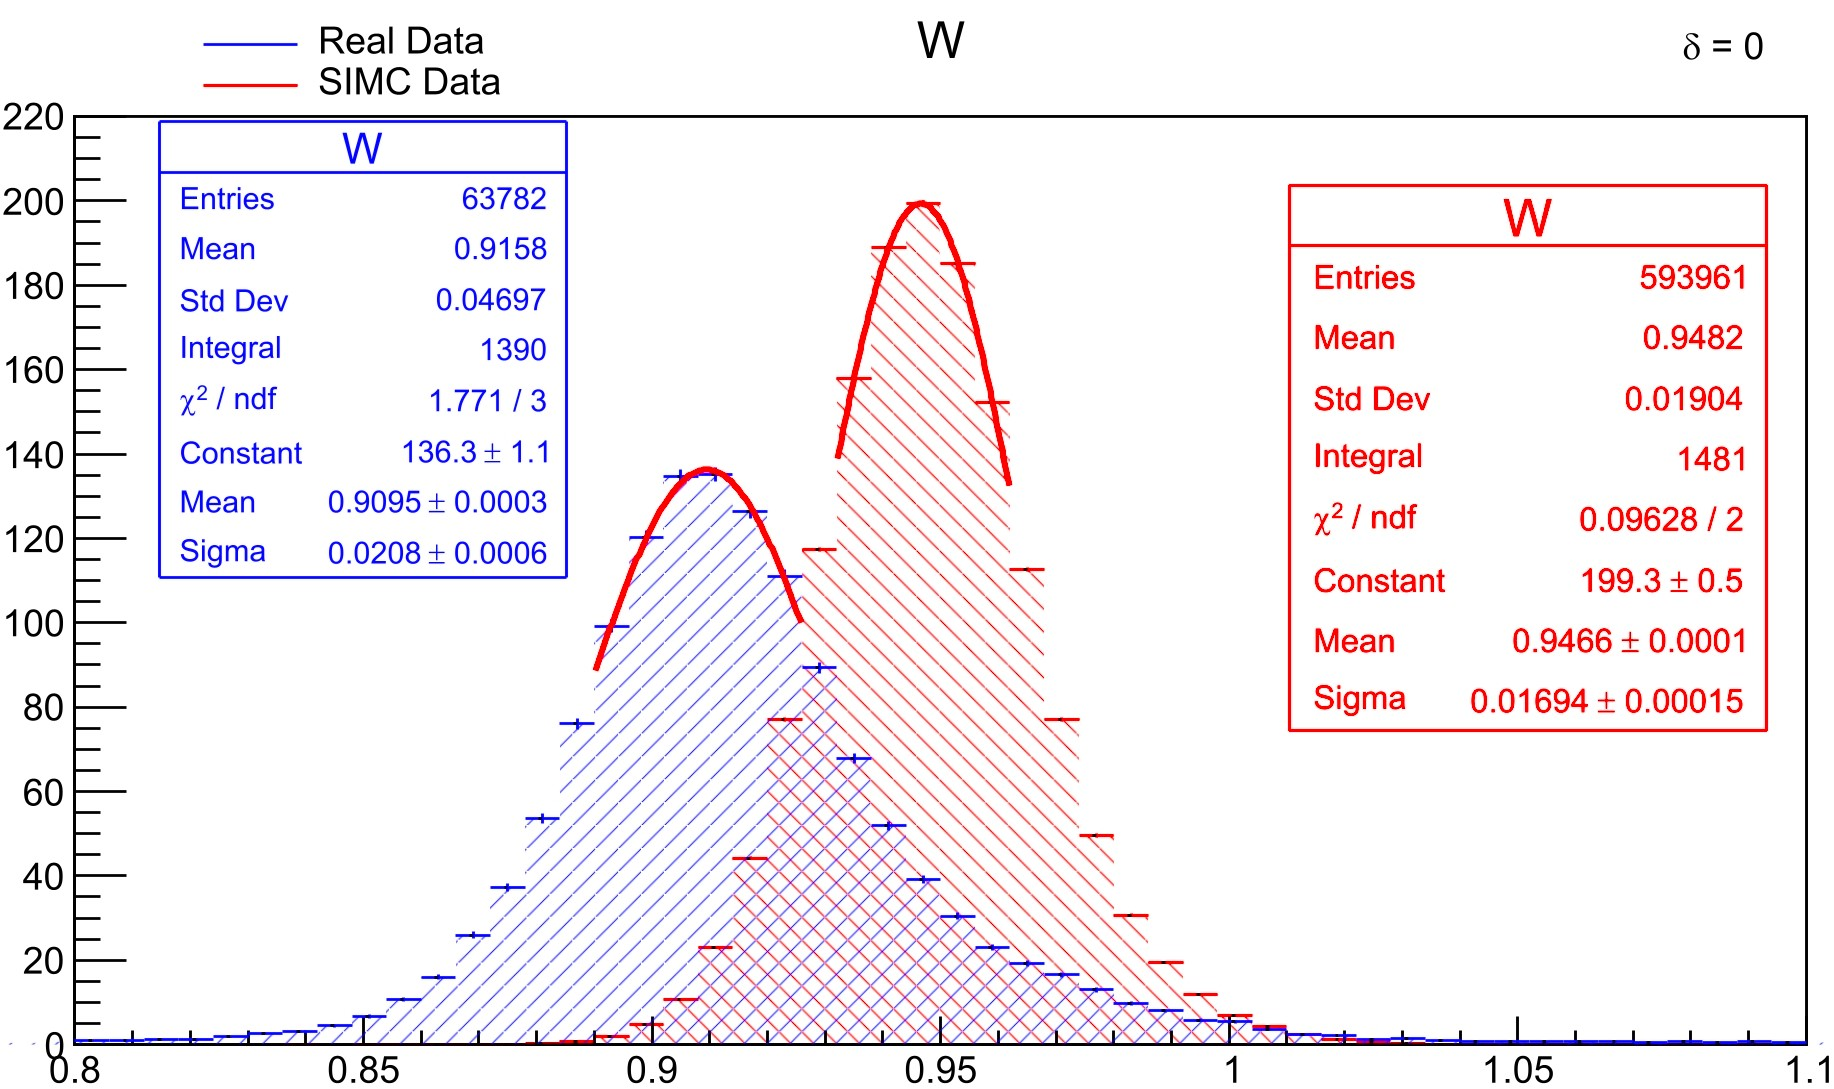
\includegraphics[width=\linewidth]{uncalibrated data/W_0.jpg}
  \end{minipage}
  \hfill
  \begin{minipage}[t]{0.5\textwidth}
    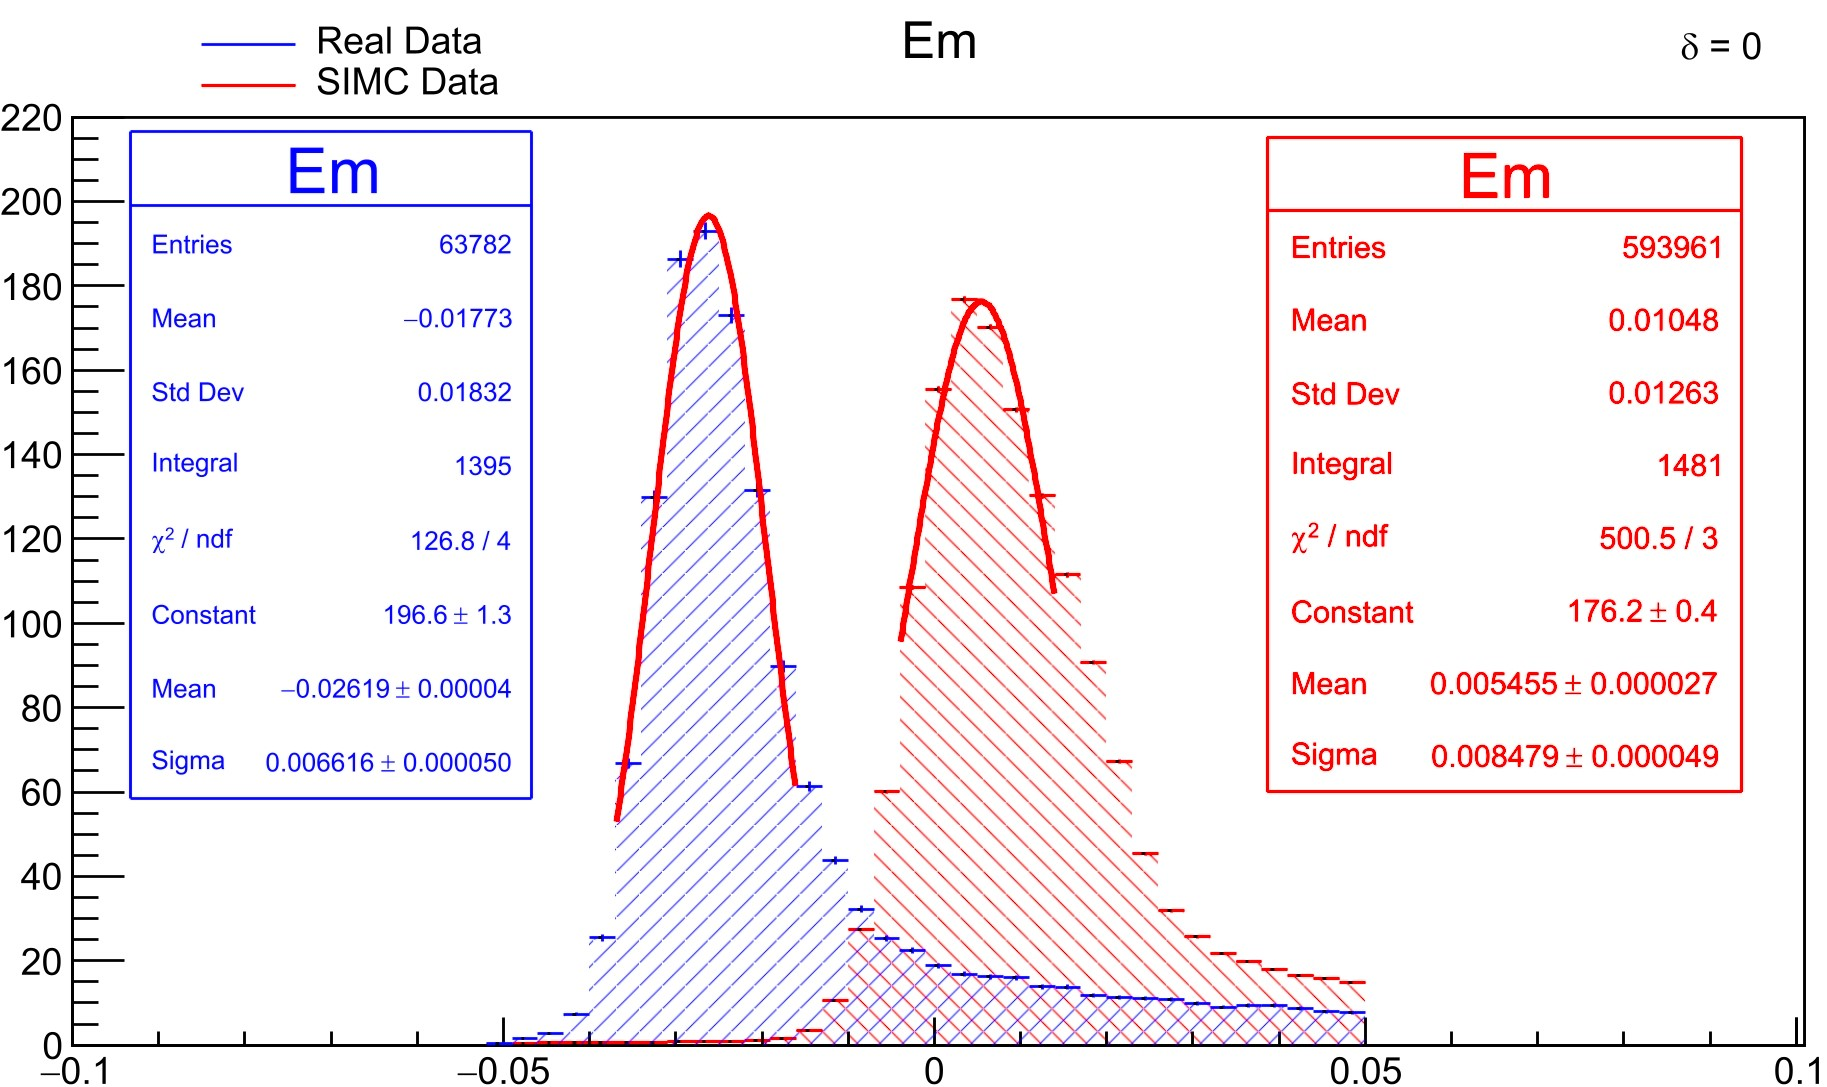
\includegraphics[width=\linewidth]{uncalibrated data/Em_0.jpg}
  \end{minipage}

  \vspace{0cm}  % Space between rows

 \begin{minipage}[t]{0.3\textwidth}
    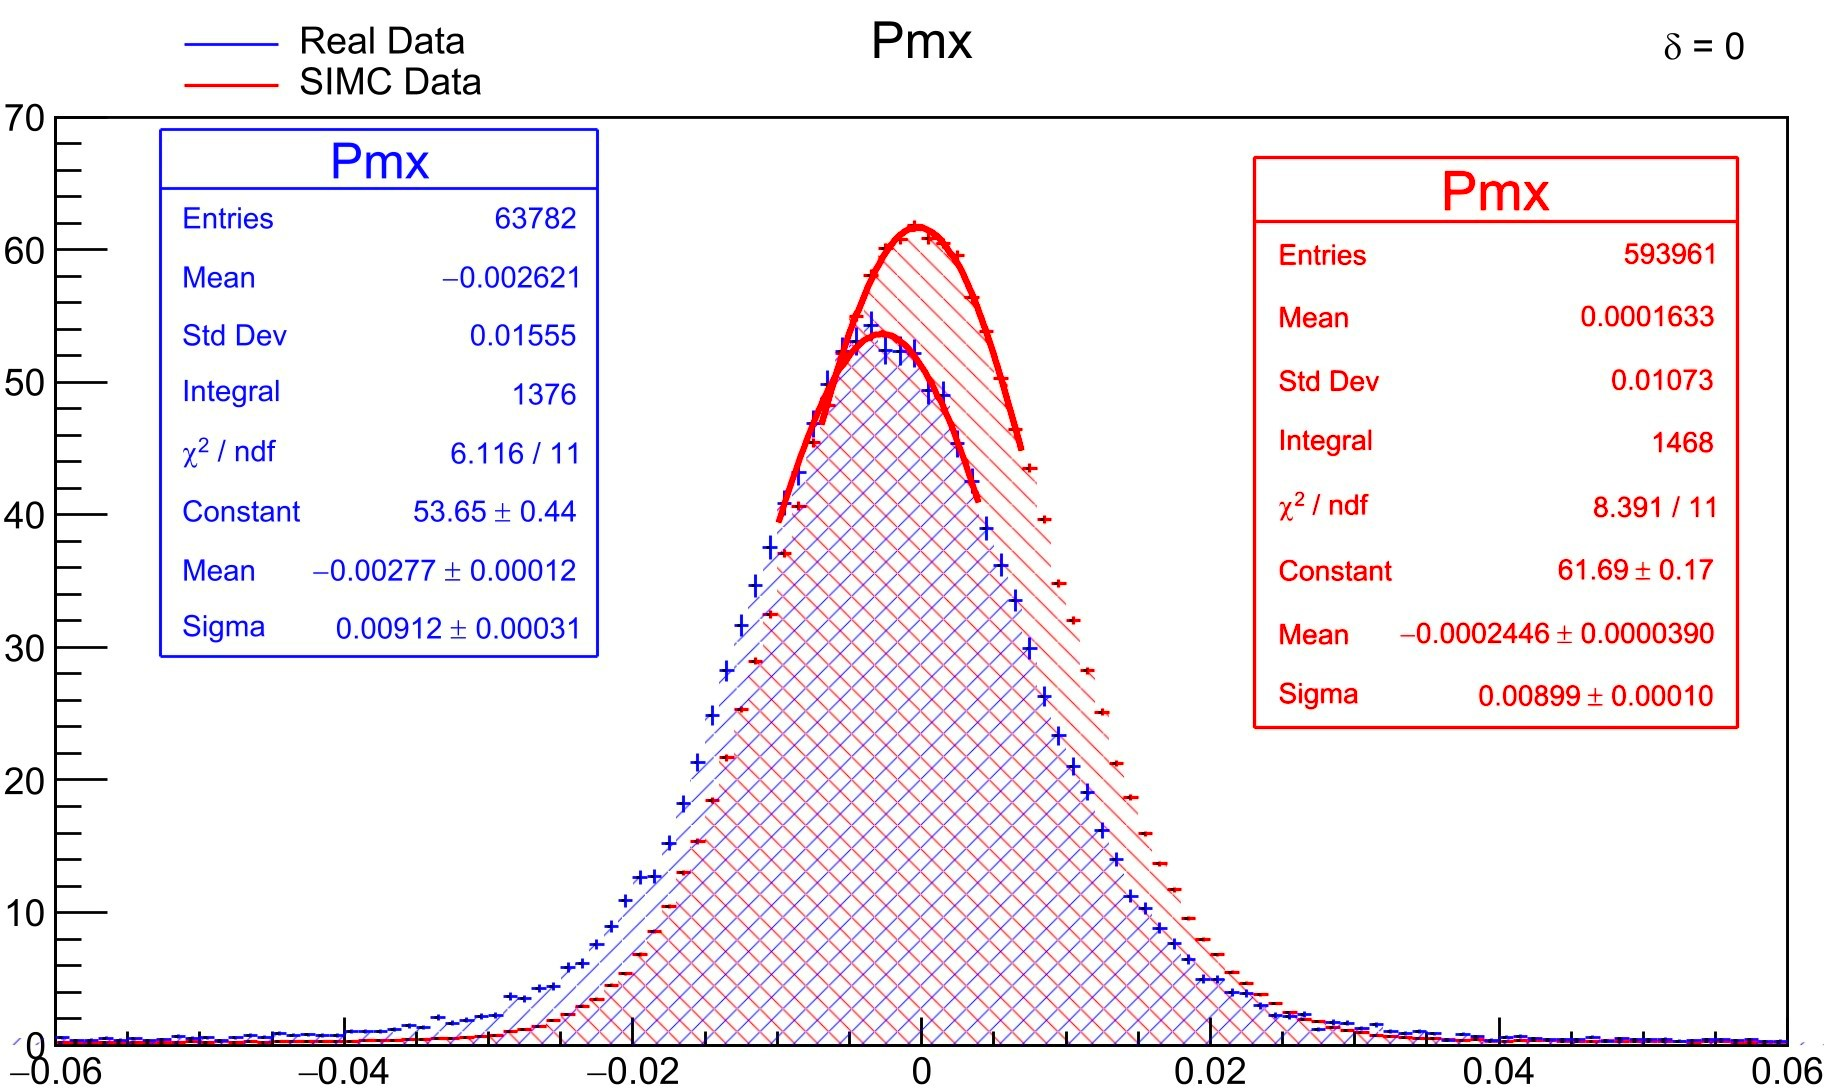
\includegraphics[width=\linewidth]{uncalibrated data/Pmx_0.jpg}
  \end{minipage}
  \begin{minipage}[t]{0.3\textwidth}
    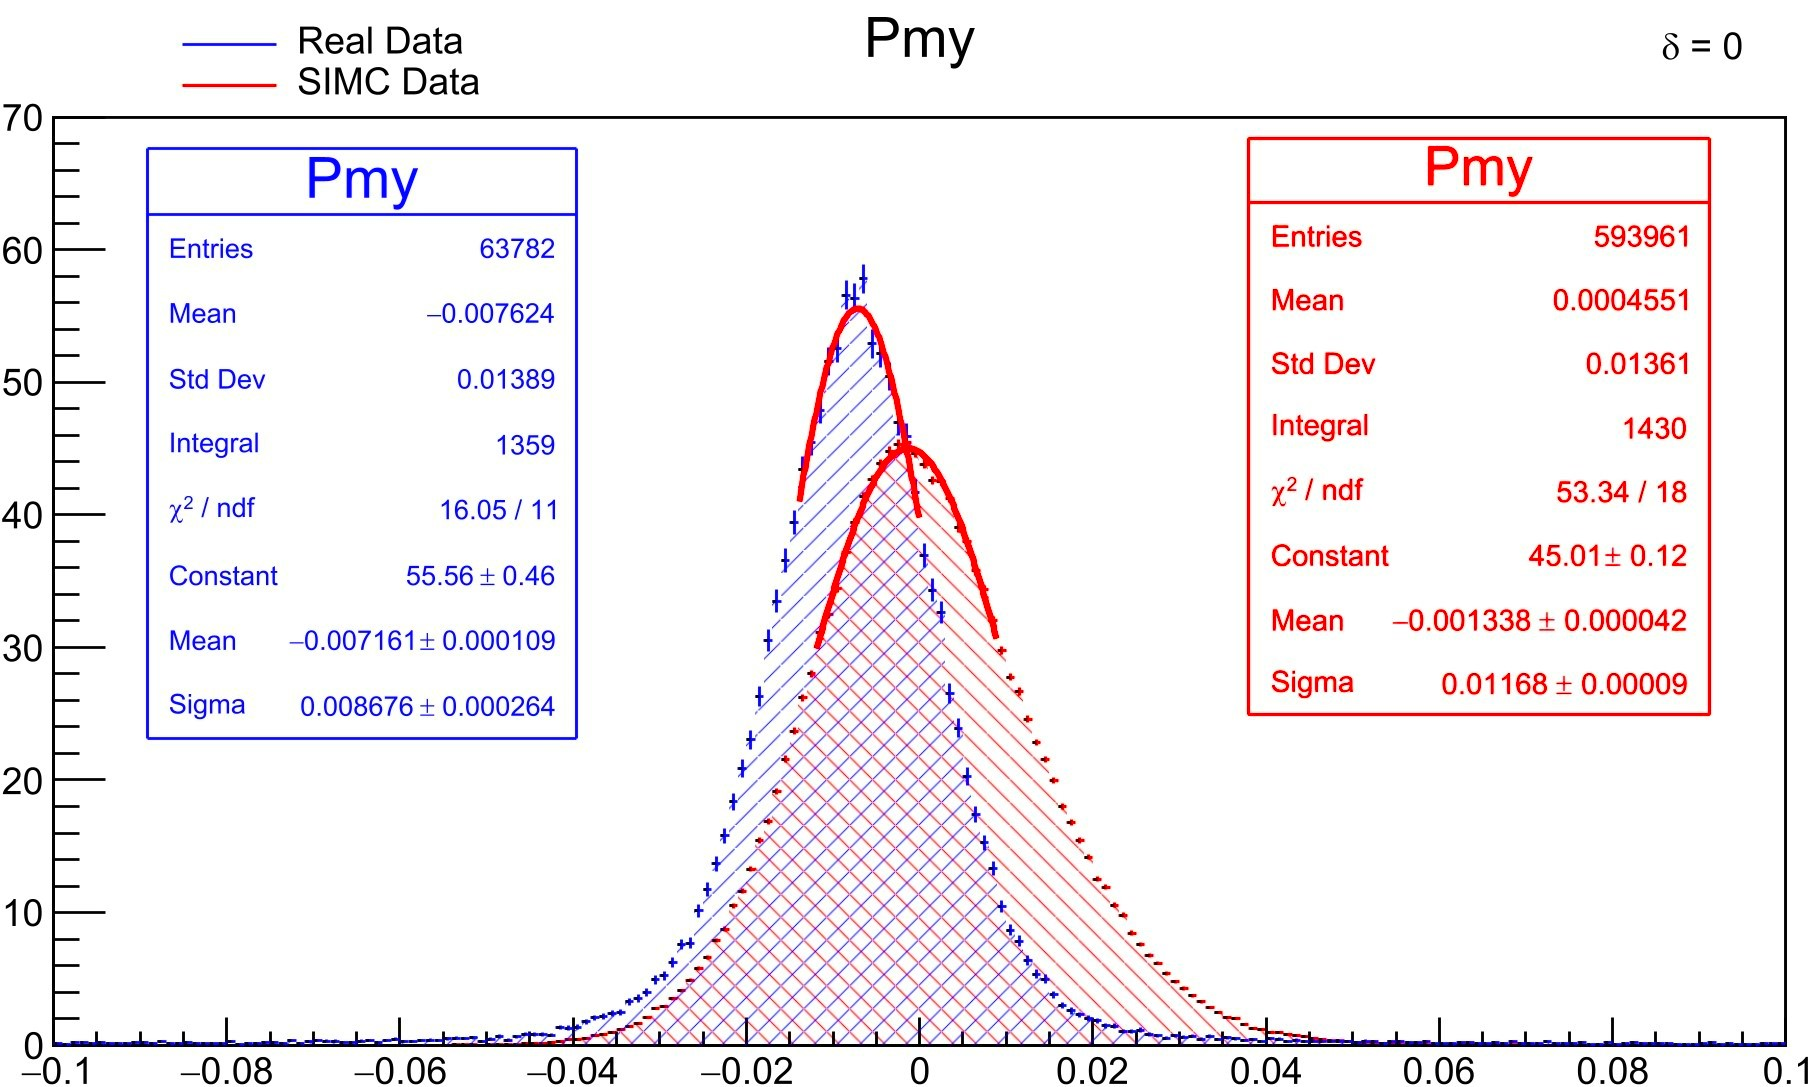
\includegraphics[width=\linewidth]{uncalibrated data/Pmy_0.jpg}
  \end{minipage}
  \begin{minipage}[t]{0.3\textwidth}
    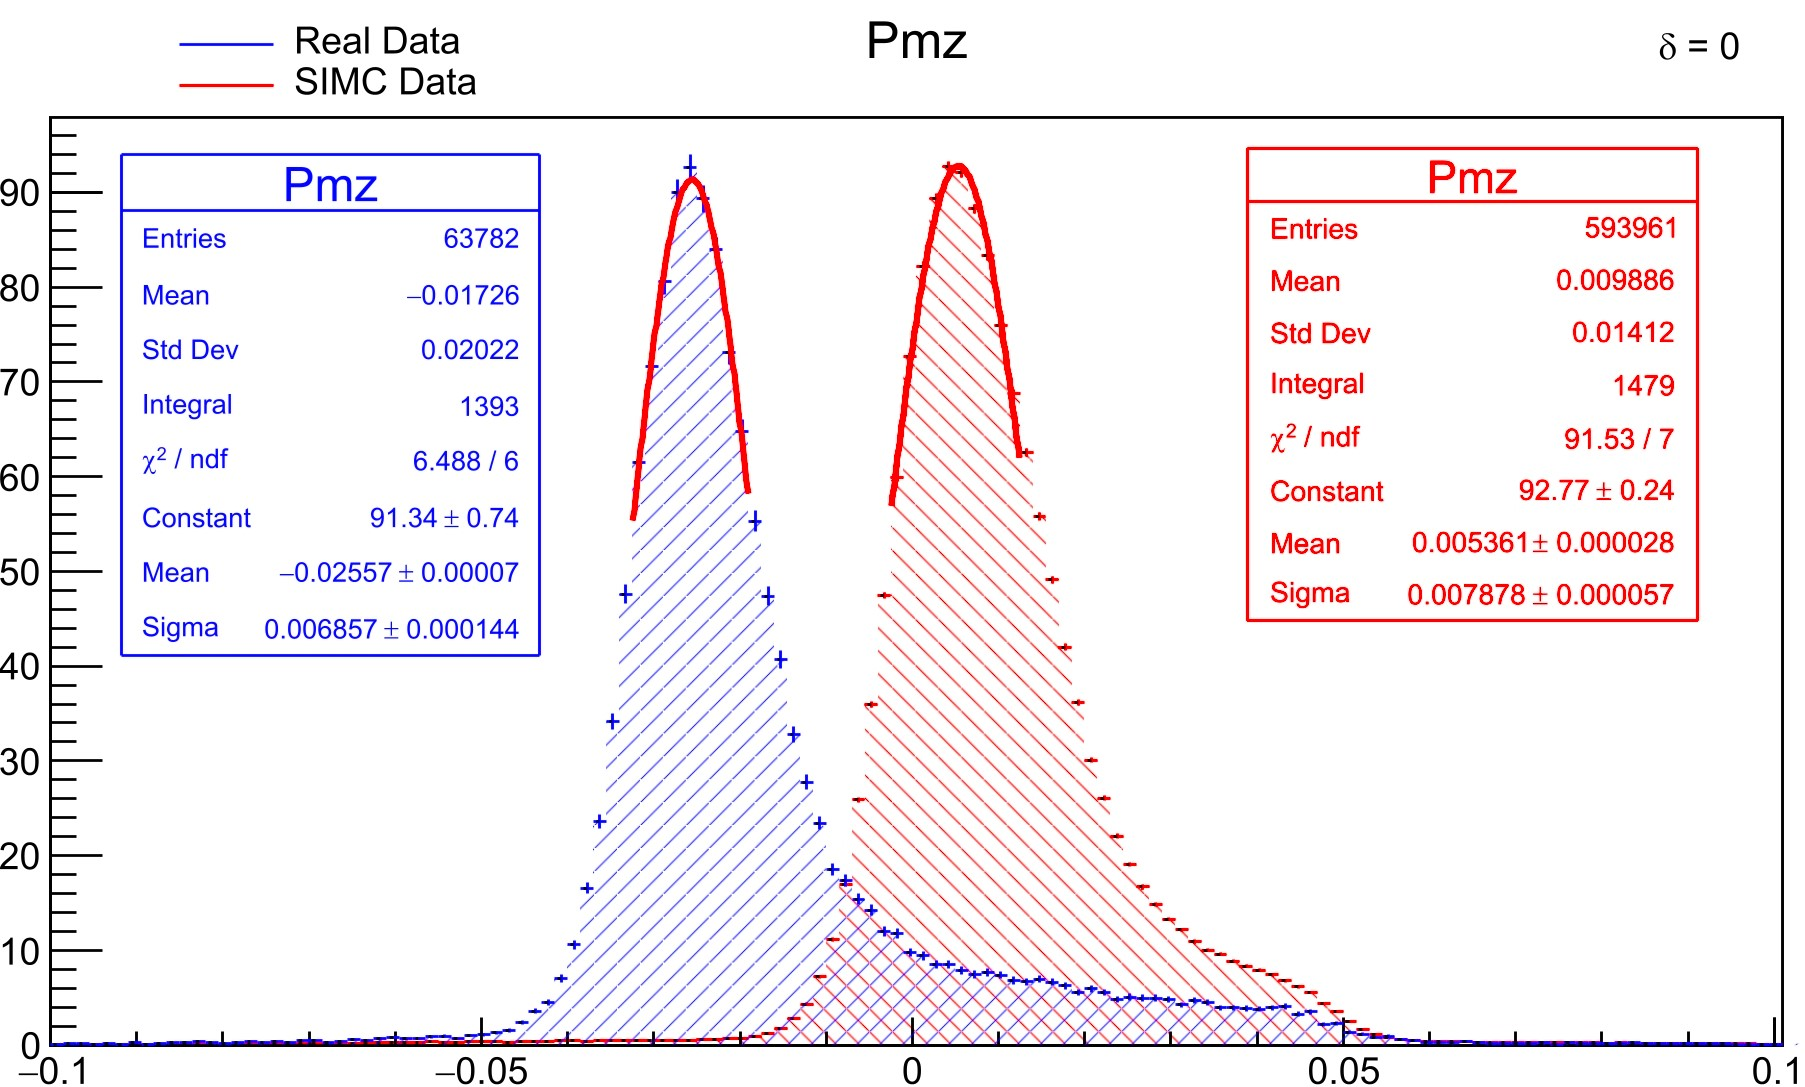
\includegraphics[width=\linewidth]{uncalibrated data/Pmz_0.jpg}
  \end{minipage}
\vspace{-1cm}
  \caption{Unoptimized spectra for $W$, $E_m$, $P_{mx}$, $P_{my}$, and $P_{mz}$ where $\delta = 0$.}
\end{figure}
\vspace{-1cm}

\end{block}


\begin{exampleblock}{Optimization Mathematics}
\begin{itemize}
    \item $\mathbb{M}\vec{x}=\vec{y}+\hat\epsilon$, where $\mathbb{M}$ is the model matrix, $\vec{x}$ is the optimized parameter vector, $\vec{y}$ is the difference between simulated and observed kinematic variables, and $\hat\epsilon$ is the residual vector.
    \item The model matrix $\mathbb{M}$ contains derivatives of kinematic variables with respect to spectrometer offsets.
    \item  The SHMS and HMS are optimized by minimizing $\hat\epsilon$.
    \item $\scriptsize \chi^2=\sum\limits_{i}\frac{(O_{obs}-C_{calc})^2}{\sigma^2_i}$, where $O_{obs}$ is the observed value, $C_{calc}$ is the calculated value, and $\sigma_{i}$ is the uncertainty of the variable.
    \item In matrix form, $\chi^2$ becomes $\chi^2=\hat\epsilon^T\mathbb{N}^{-1}\hat\epsilon$, where $\mathbb{N}$ is a diagonal covariant matrix with the uncertainties of each kinematic variable (assuming uncorrelated measurement errors).
    \item The optimal solution satisfies $\frac{\partial \chi^2}{\partial \vec{x}}=0$, leading to the equation $ \vec{x}=(\mathbb{M}^T\mathbb{N}^{-1}\mathbb{M})^{-1}\mathbb{M}^T\mathbb{N}^{-1}\vec{y}$.
    \item All calculations are automated using Python.
\end{itemize}

\begin{figure}
\vspace{-1.5cm}$$\Large\begin{pmatrix}
E_f \frac{\partial W}{\partial E_f} & \frac{\partial W}{\partial \theta_e} & \frac{\partial W}{\partial \theta_p} & \frac{\partial W}{\partial \phi_e} & \frac{\partial W}{\partial \phi_p} & P_p \frac{\partial W}{\partial P_p} \\
E_f \frac{\partial E_m}{\partial E_f} & \frac{\partial E_m}{\partial \theta_e} & \frac{\partial E_m}{\partial \theta_p} & \frac{\partial E_m}{\partial \phi_e} & \frac{\partial E_m}{\partial \phi_p} & P_p \frac{\partial E_m}{\partial P_p} \\
E_f \frac{\partial P_{mx}}{\partial E_f} & \frac{\partial P_{mx}}{\partial \theta_e} & \frac{\partial P_{mx}}{\partial \theta_p} & \frac{\partial P_{mx}}{\partial \phi_e} & \frac{\partial P_{mx}}{\partial \phi_p} & P_p \frac{\partial P_{mx}}{\partial P_p} \\
E_f \frac{\partial P_{my}}{\partial E_f} & \frac{\partial P_{my}}{\partial \theta_e} & \frac{\partial P_{my}}{\partial \theta_p} & \frac{\partial P_{my}}{\partial \phi_e} & \frac{\partial P_{my}}{\partial \phi_p} & P_p \frac{\partial P_{my}}{\partial P_p} \\
E_f \frac{\partial P_{mz}}{\partial E_f} & \frac{\partial P_{mz}}{\partial \theta_e} & \frac{\partial P_{mz}}{\partial \theta_p} & \frac{\partial P_{mz}}{\partial \phi_e} & \frac{\partial P_{mz}}{\partial \phi_p} & P_p \frac{\partial P_{mz}}{\partial P_p}
\end{pmatrix}\begin{pmatrix}
 \frac{\delta E_f}{E_f} \\ \delta \theta_e \\ \delta \theta_p \\ \delta \phi_e \\ \delta \phi_p \\ \frac{\delta P_p}{P_p}
\end{pmatrix}=\begin{pmatrix} dW \\ dE_m \\ dP_{mx} \\ dP_{my} \\ dP_{mz} \end{pmatrix}+\begin{pmatrix} \hat{\epsilon}_{dW} \\ \hat{\epsilon}_{dE_m} \\ \hat{\epsilon}_{P_{mx}} \\ \hat{\epsilon}_{P_{my}} \\ \hat{\epsilon}_{P_{mz}} \end{pmatrix}
$$
\vspace{-1cm}
\caption{The equation $\mathbb{M}\vec{x}=\vec{y}+\hat\epsilon$ for Model 3 fully illustrated for a single run.}
\end{figure}    

\end{exampleblock}

\end{column}

\separatorcolumn

\begin{column}{\colwidth}
\vspace{-0.5cm}
\begin{block}{Optimized Data}
\vspace{-.5cm}
\begin{figure}
  \centering

  % Top row: 3 plots
  \begin{minipage}[t]{0.49\textwidth}
    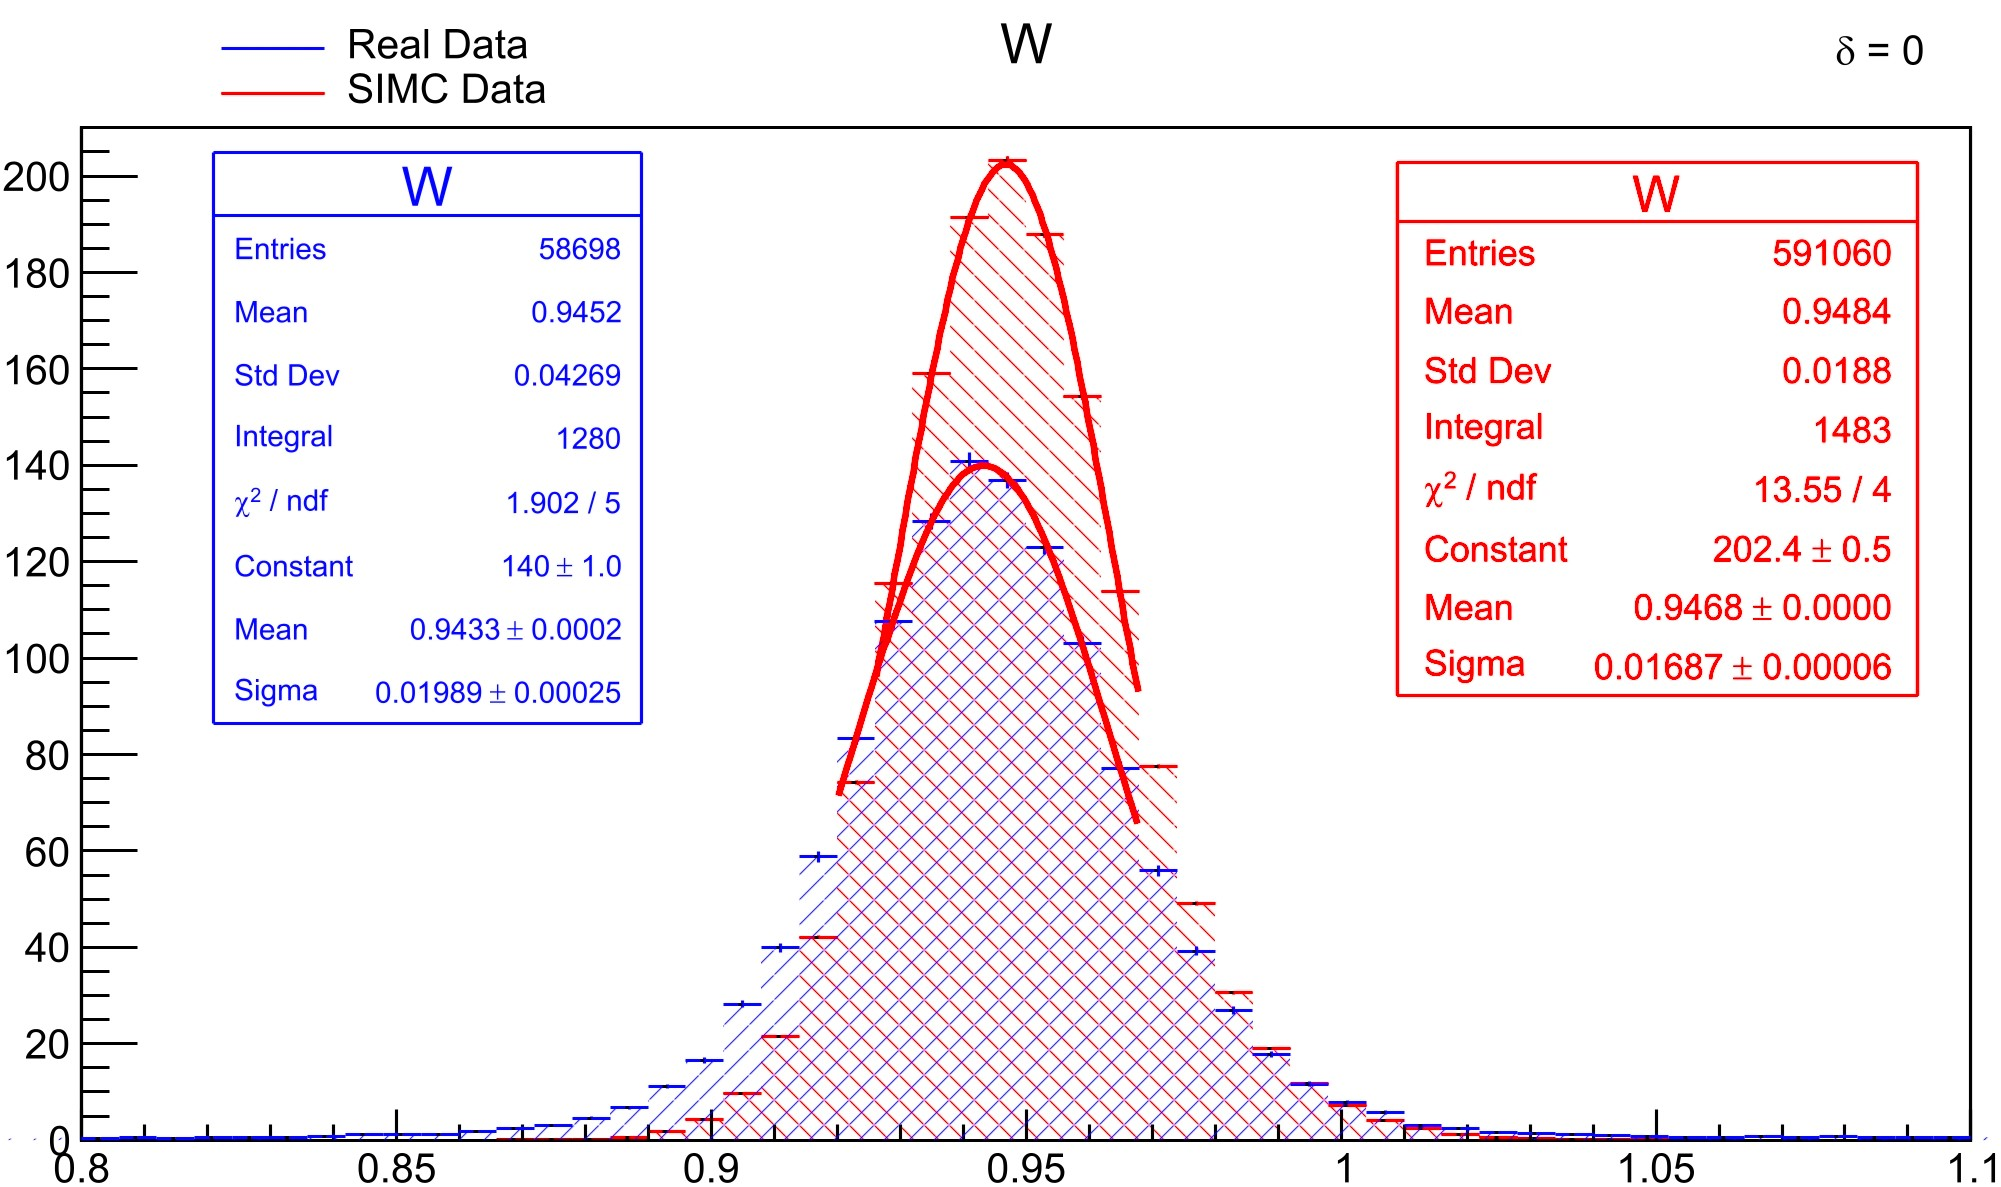
\includegraphics[width=\linewidth]{calibrated data/model 0/W_0.jpg}
  \end{minipage}
  \hfill
  \begin{minipage}[t]{0.5\textwidth}
    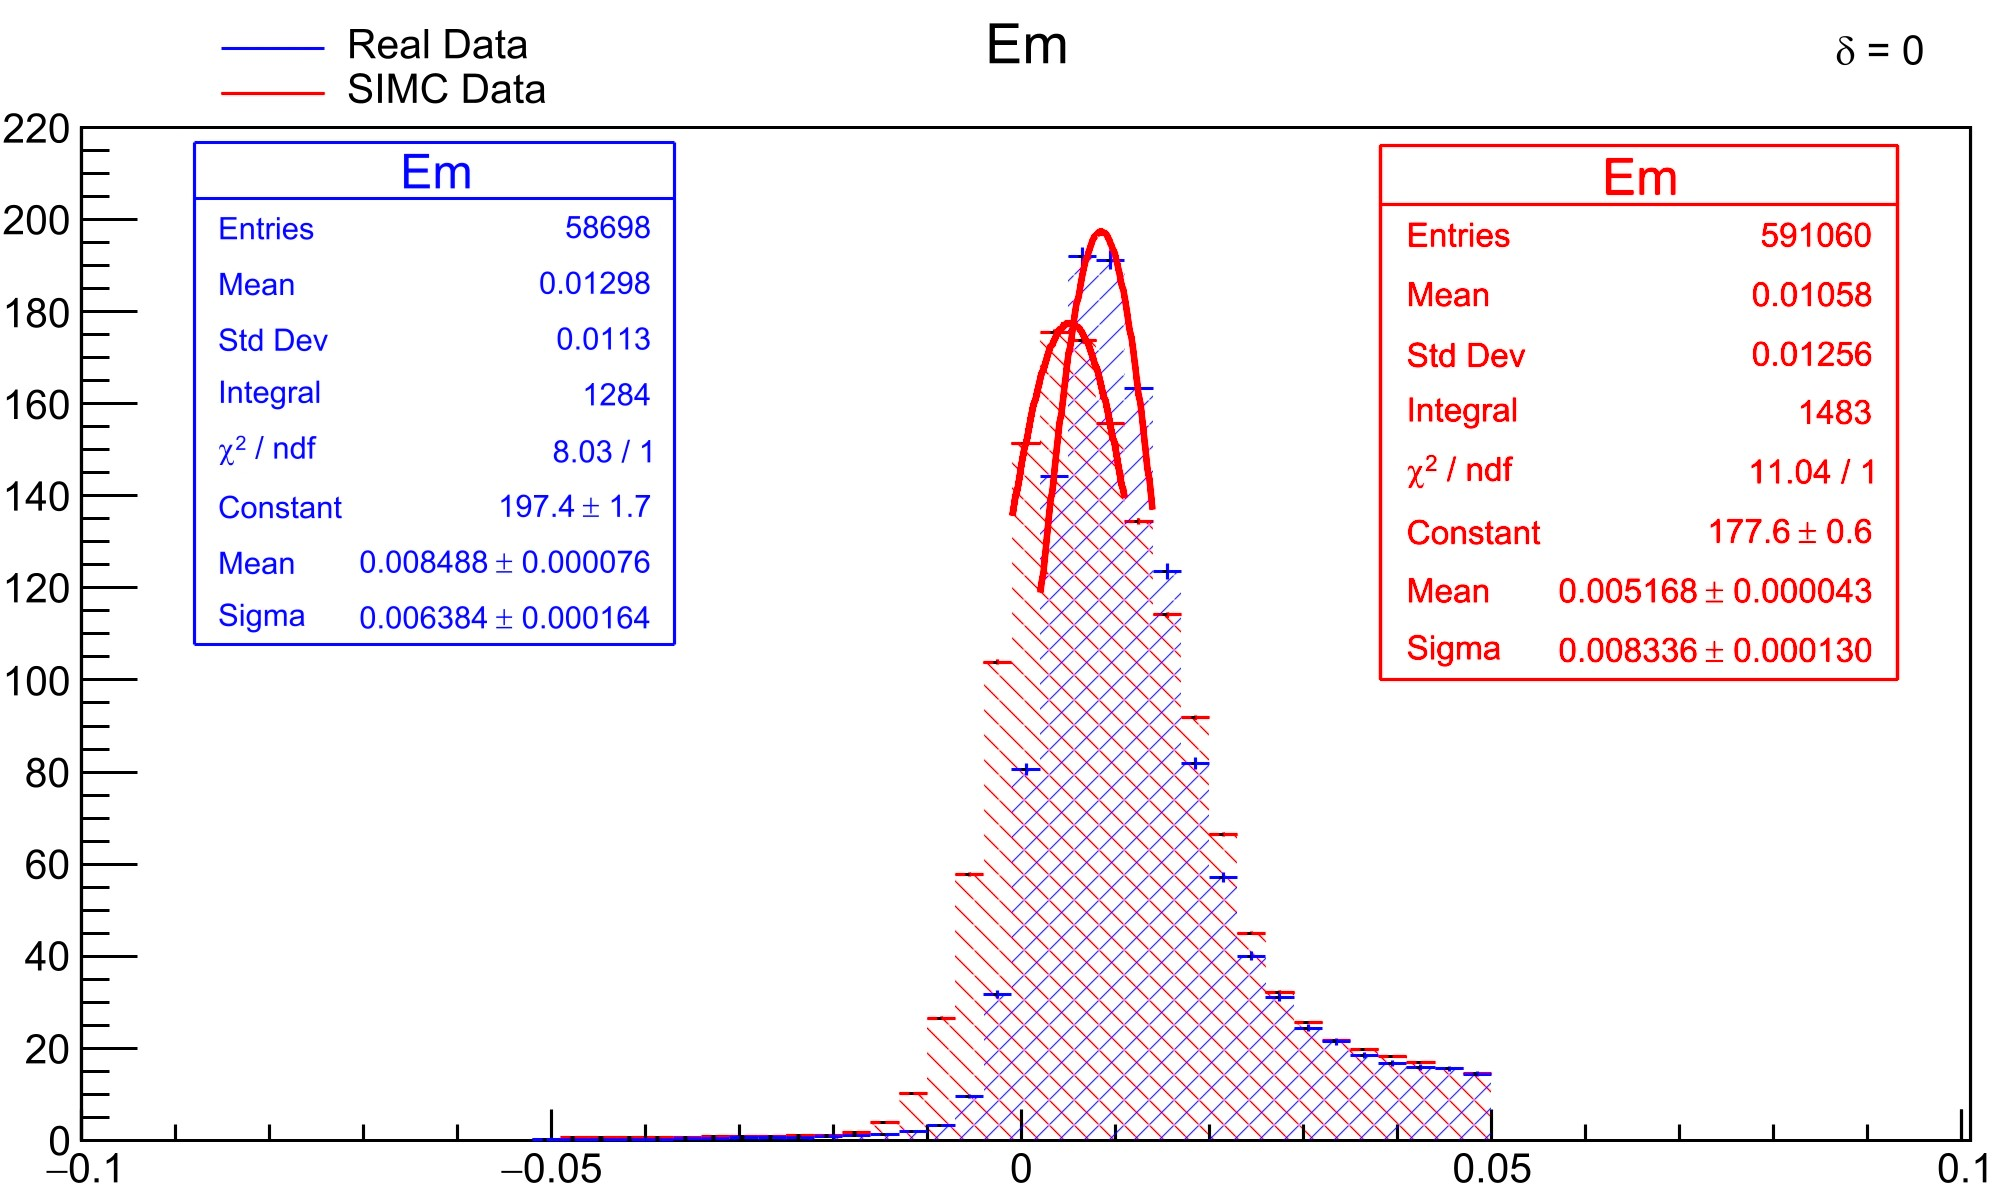
\includegraphics[width=\linewidth]{calibrated data/model 0/Em_0.jpg}
  \end{minipage}

  \vspace{0cm}  % Space between rows

 \begin{minipage}[t]{0.3\textwidth}
    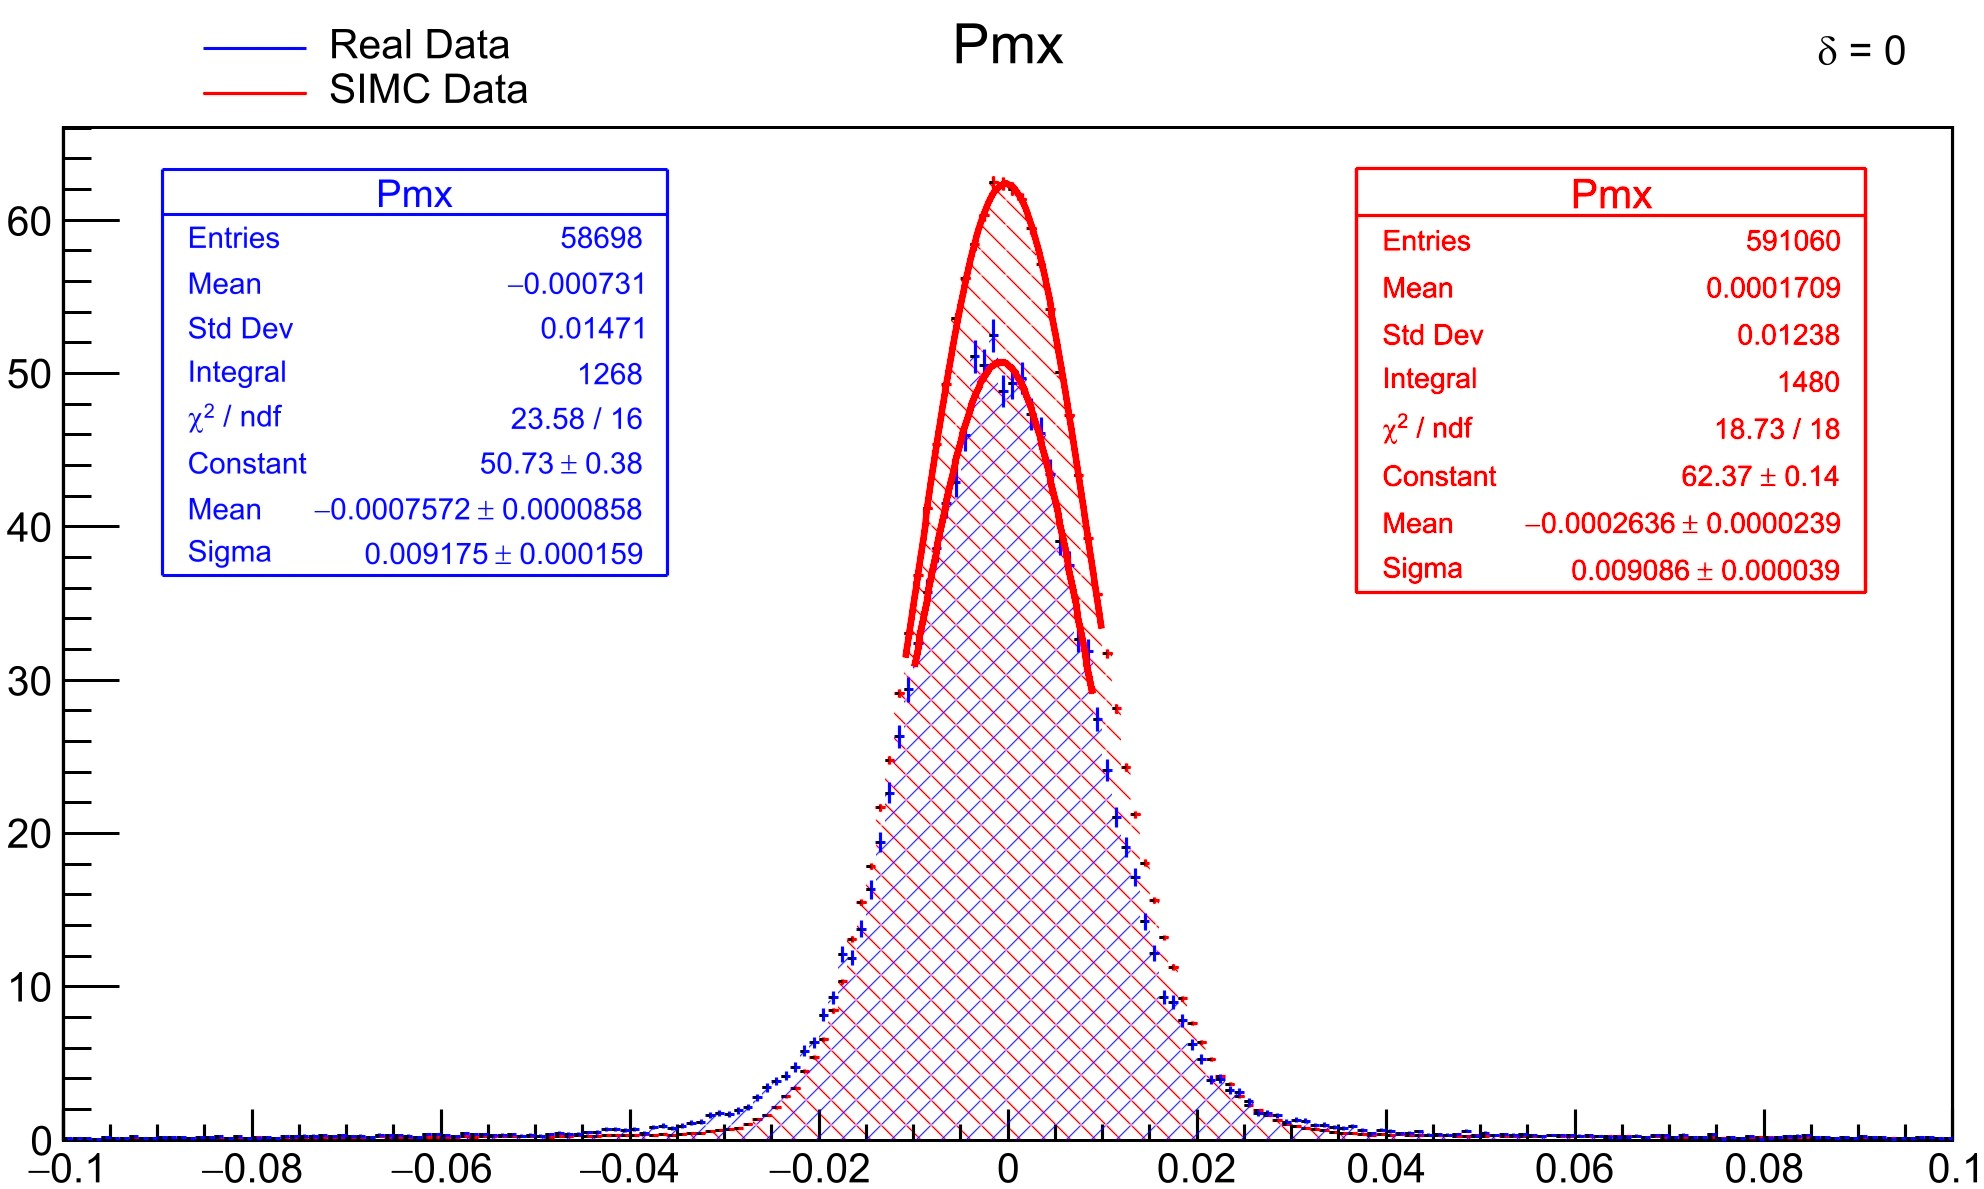
\includegraphics[width=\linewidth]{calibrated data/model 0/Pmx_0.jpg}
  \end{minipage}
  \begin{minipage}[t]{0.3\textwidth}
    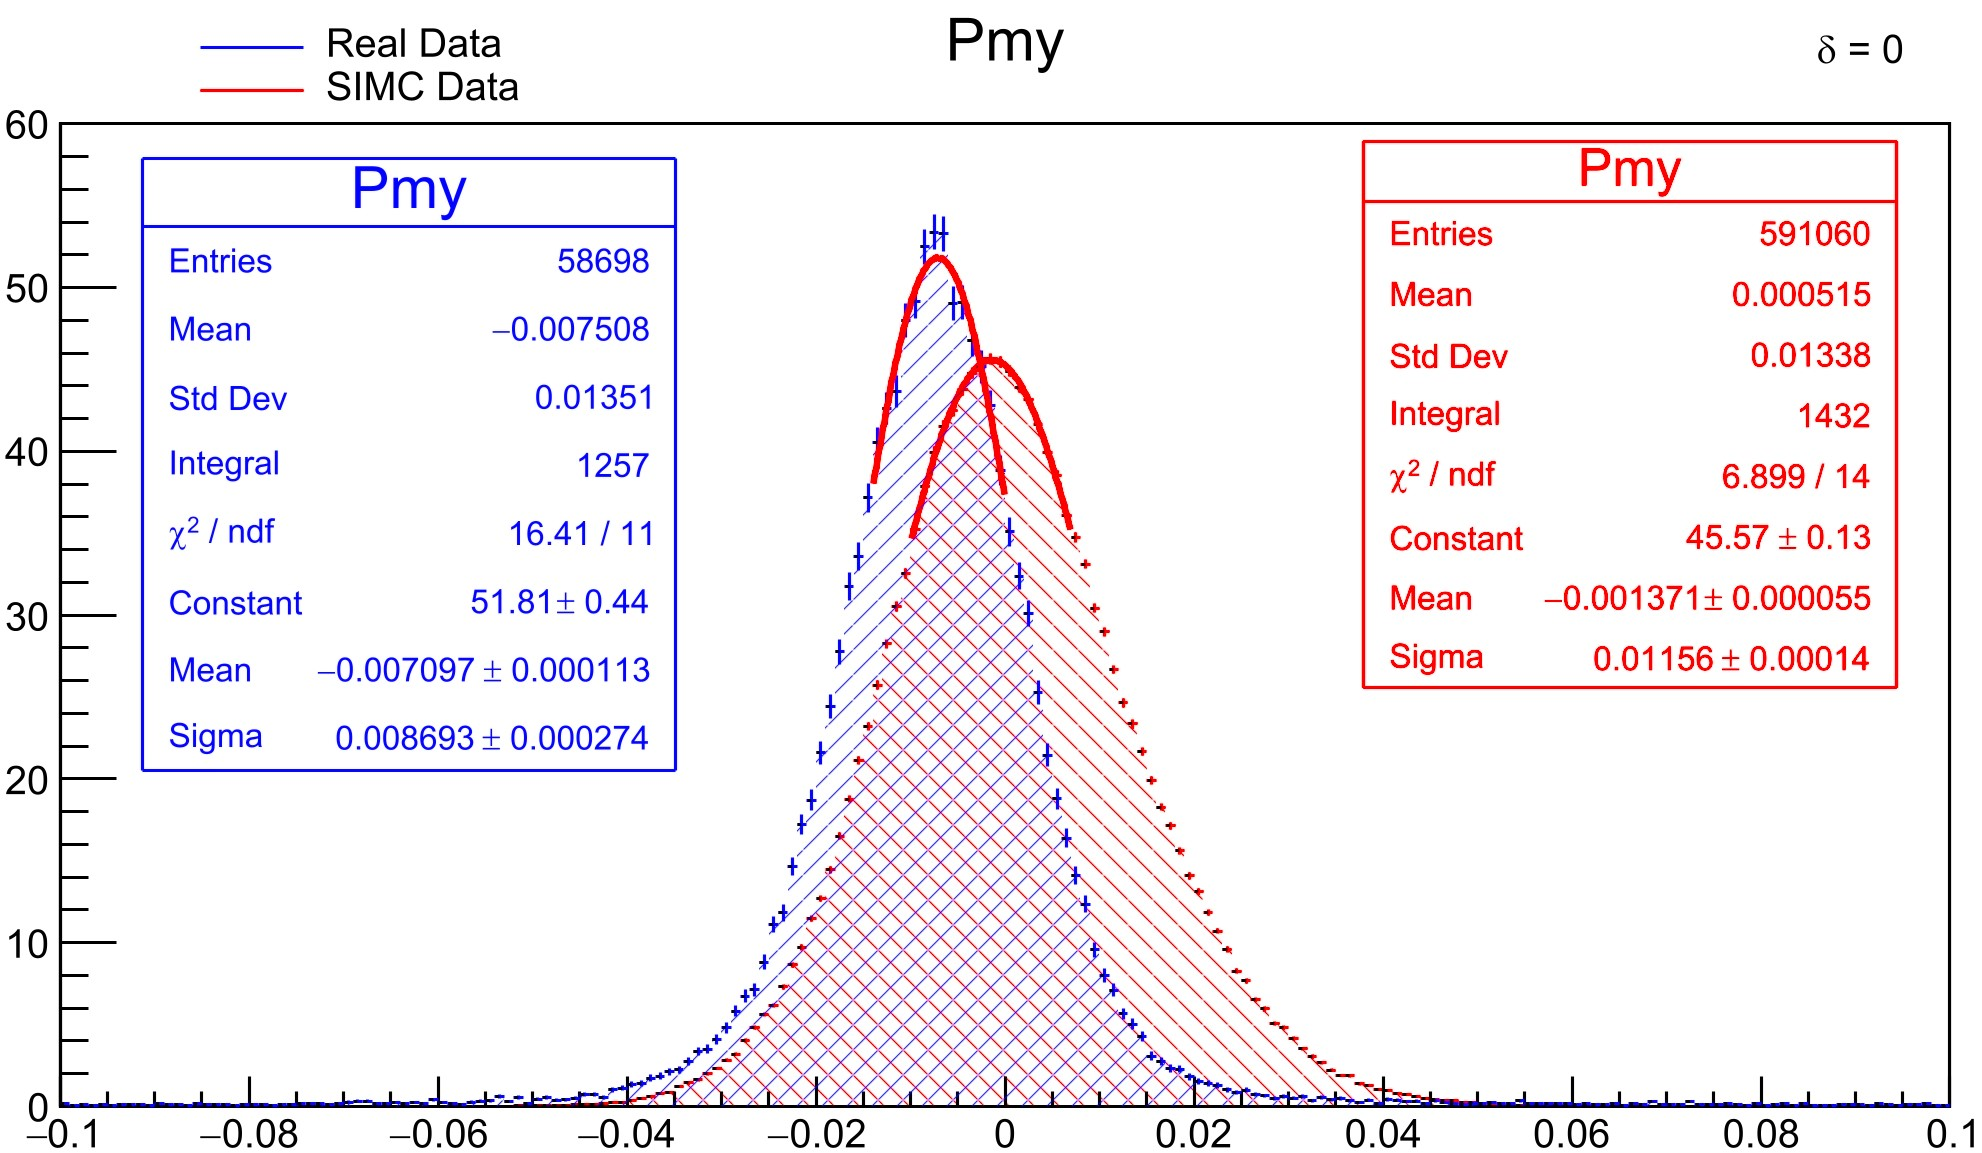
\includegraphics[width=\linewidth]{calibrated data/model 0/Pmy_0.jpg}
  \end{minipage}
  \begin{minipage}[t]{0.3\textwidth}
    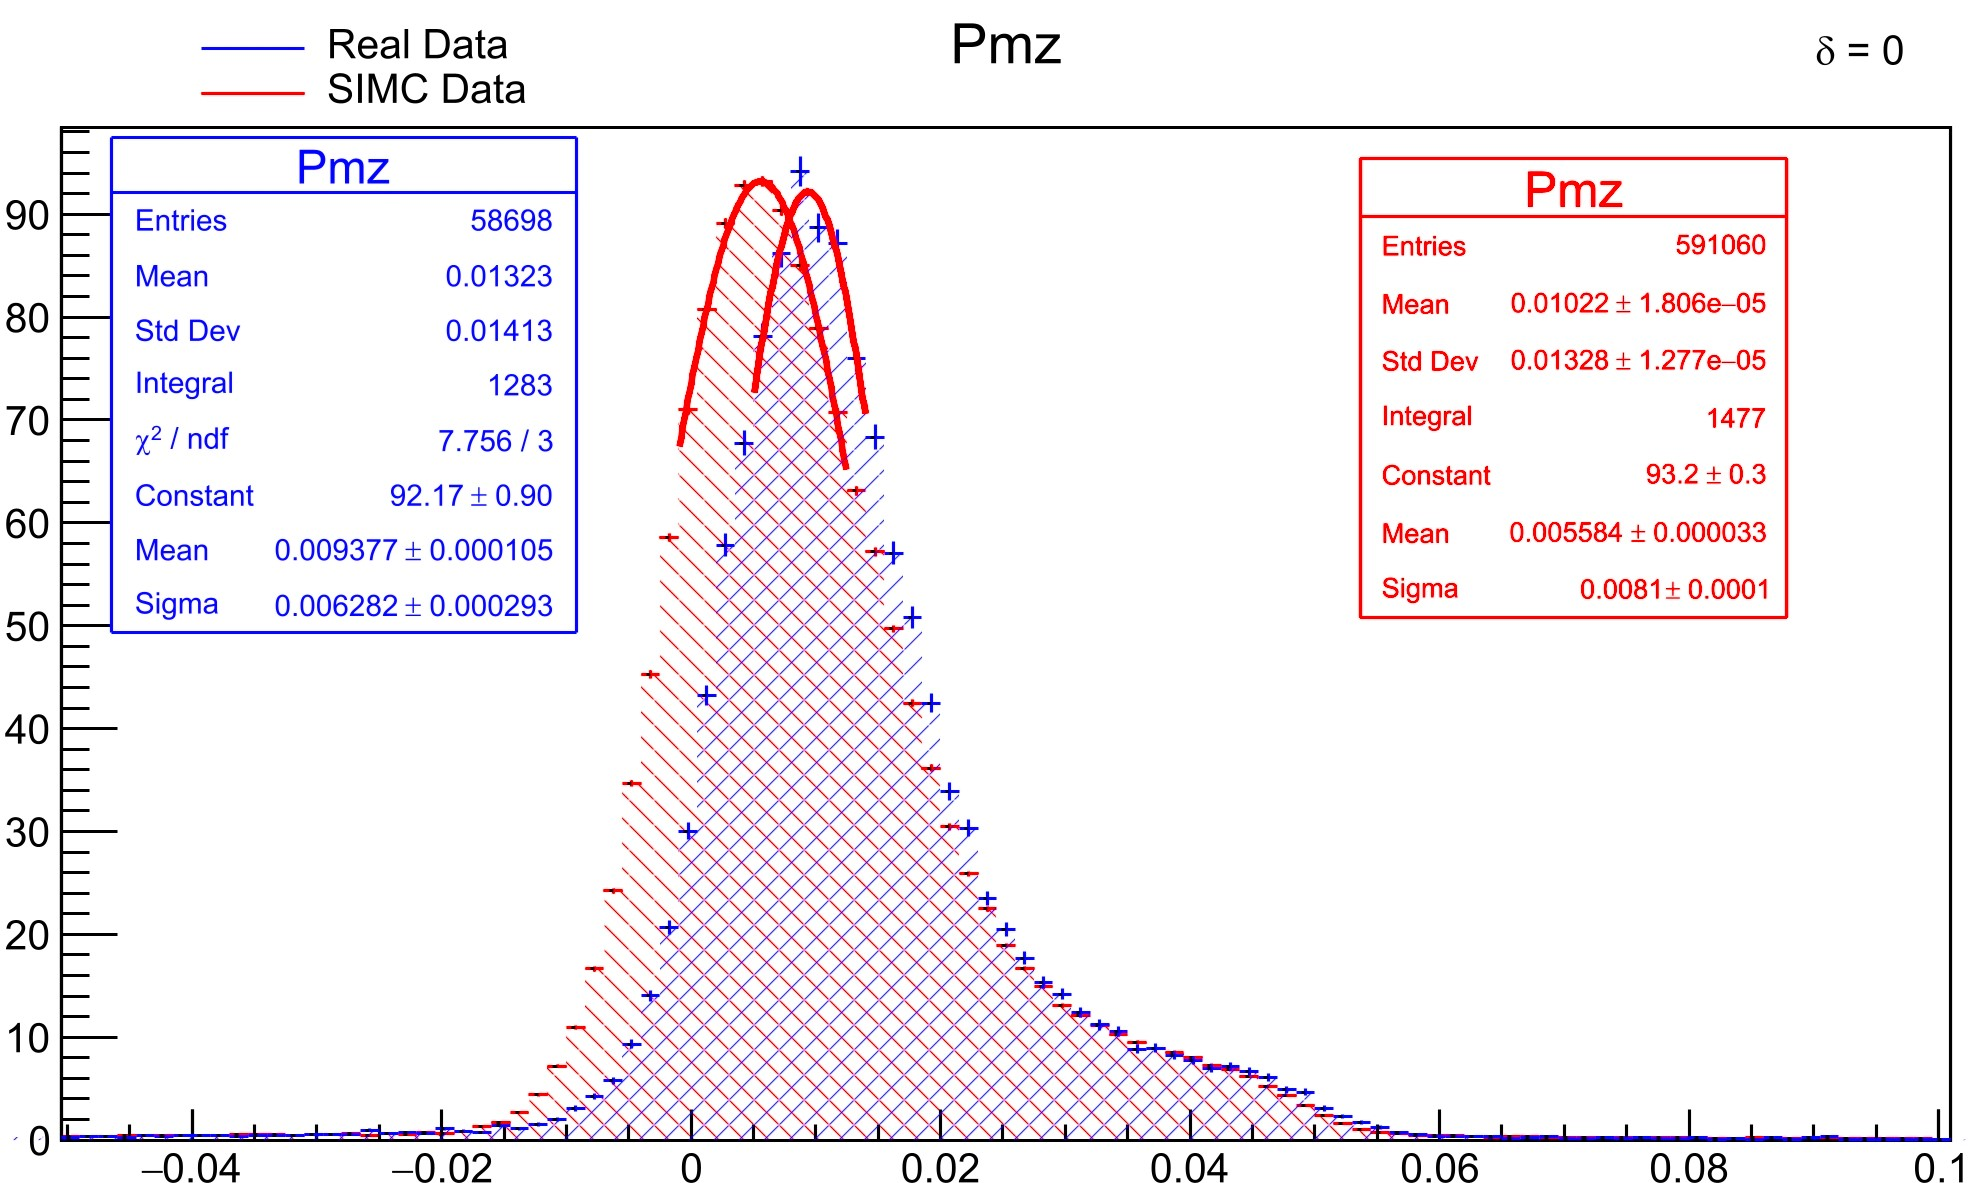
\includegraphics[width=\linewidth]{calibrated data/model 0/Pmz_0.jpg}
  \end{minipage}
\vspace{-.75cm}
  \caption{Optimized spectra for $W$, $E_m$, $P_{mx}$, $P_{my}$, and $P_{mz}$ using Model 0 offsets, deltaP $P_p$ correction on a $\delta=0$ run.}
\end{figure}

\vspace{-1.25cm}
\begin{figure}
\begin{minipage}[t]{0.49\textwidth}
    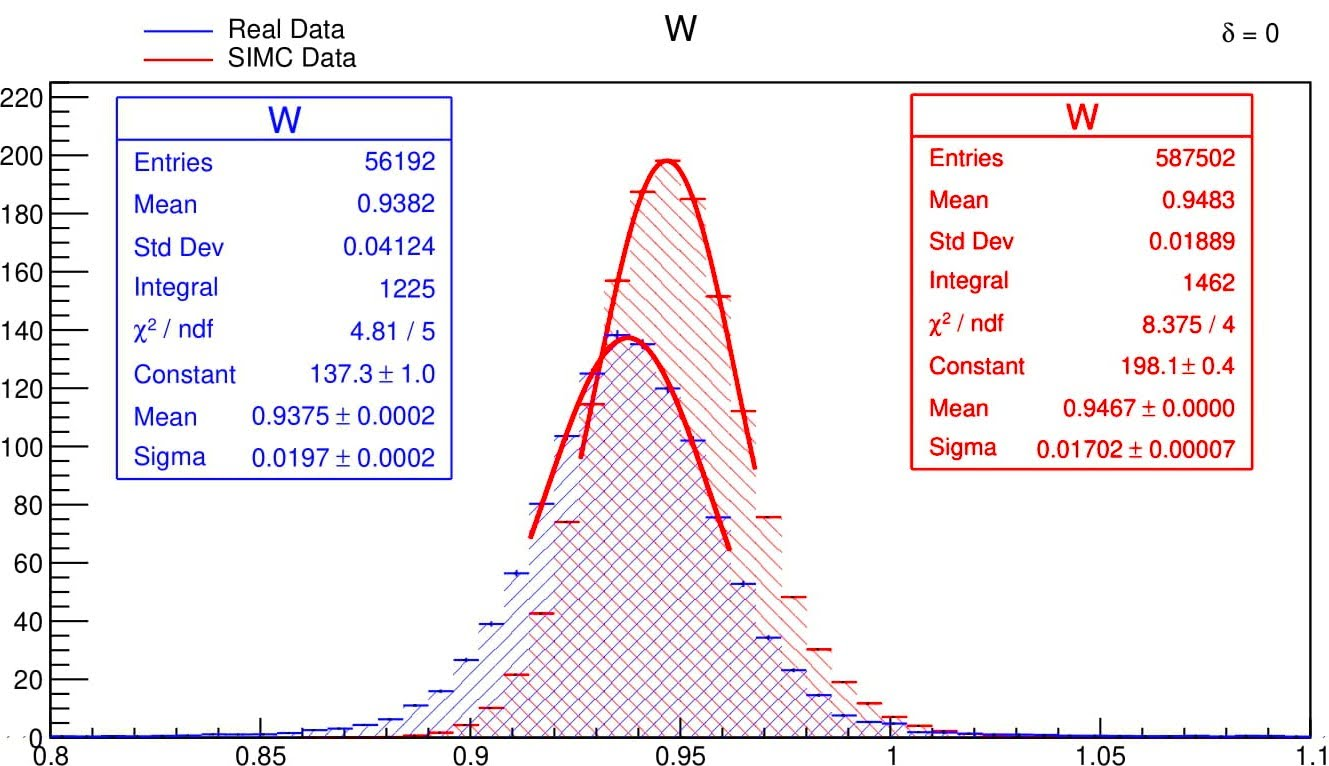
\includegraphics[width=\linewidth]{calibrated data/model 3/W_0.jpg}
  \end{minipage}
  \hfill
  \begin{minipage}[t]{0.5\textwidth}
    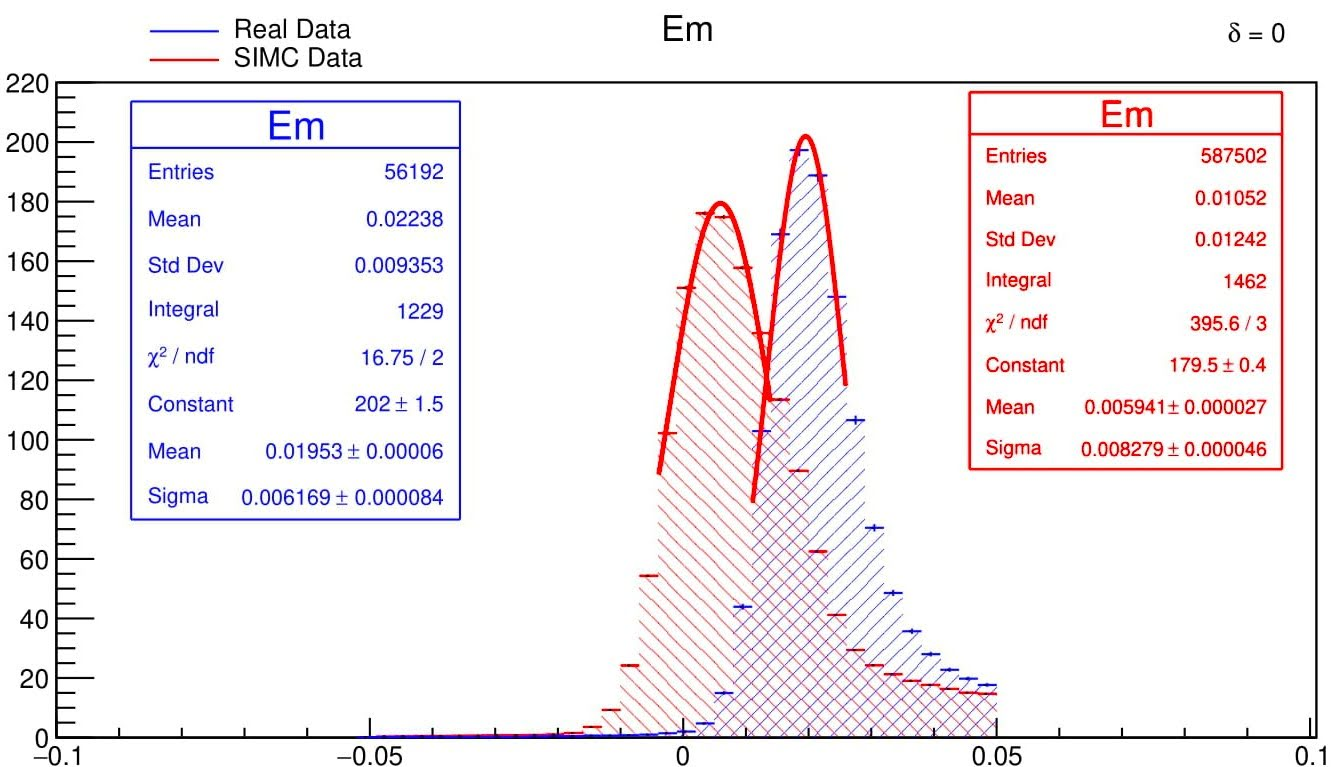
\includegraphics[width=\linewidth]{calibrated data/model 3/Em_0.jpg}
  \end{minipage}

  \vspace{0cm}  % Space between rows

 \begin{minipage}[t]{0.3\textwidth}
    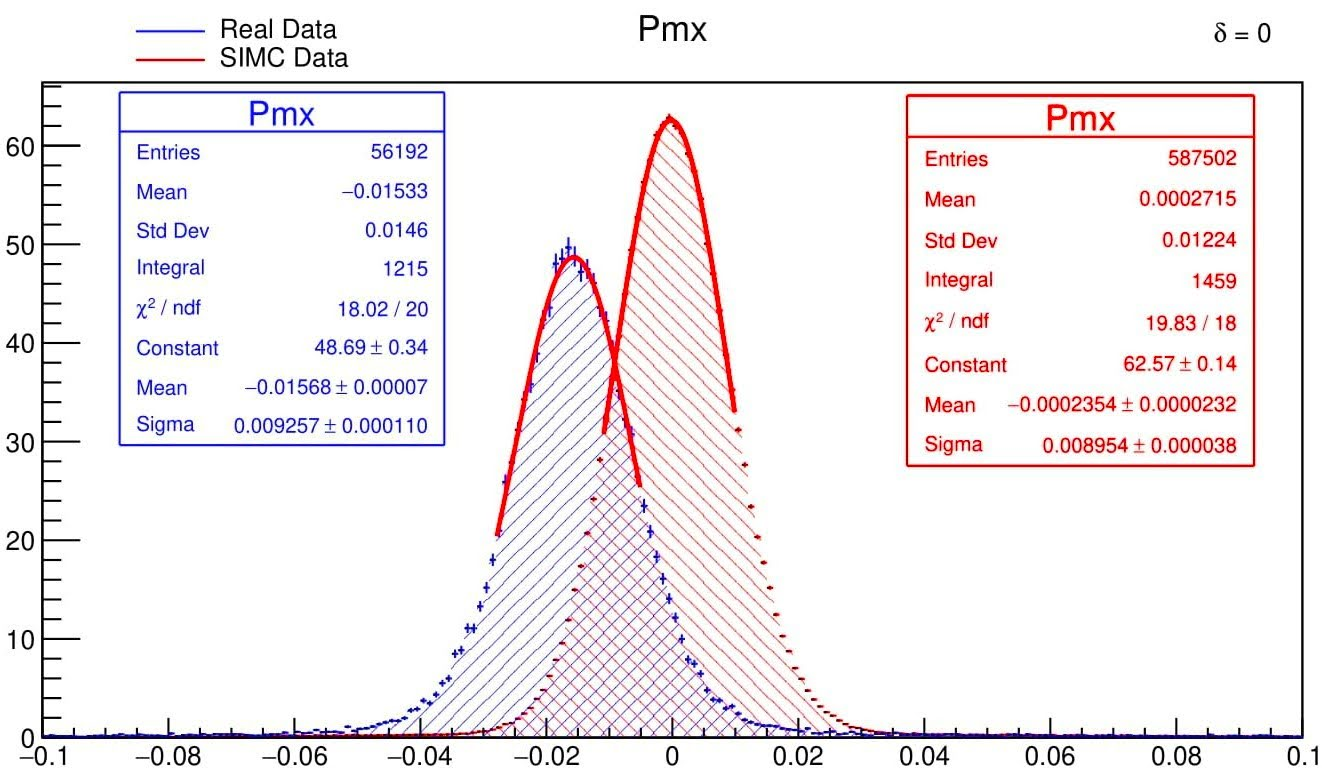
\includegraphics[width=\linewidth]{calibrated data/model 3/Pmx_0.jpg}
  \end{minipage}
  \begin{minipage}[t]{0.3\textwidth}
    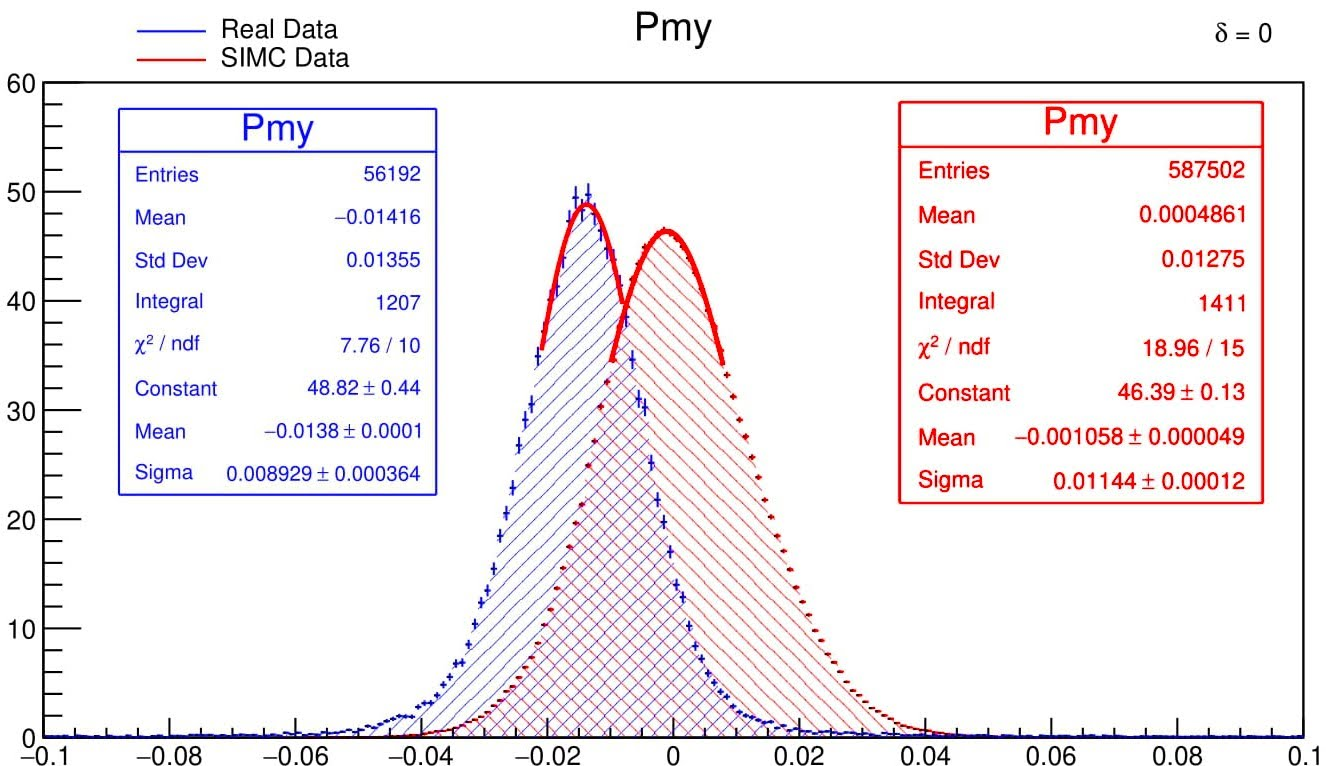
\includegraphics[width=\linewidth]{calibrated data/model 3/Pmy_0.jpg}
  \end{minipage}
  \begin{minipage}[t]{0.3\textwidth}
    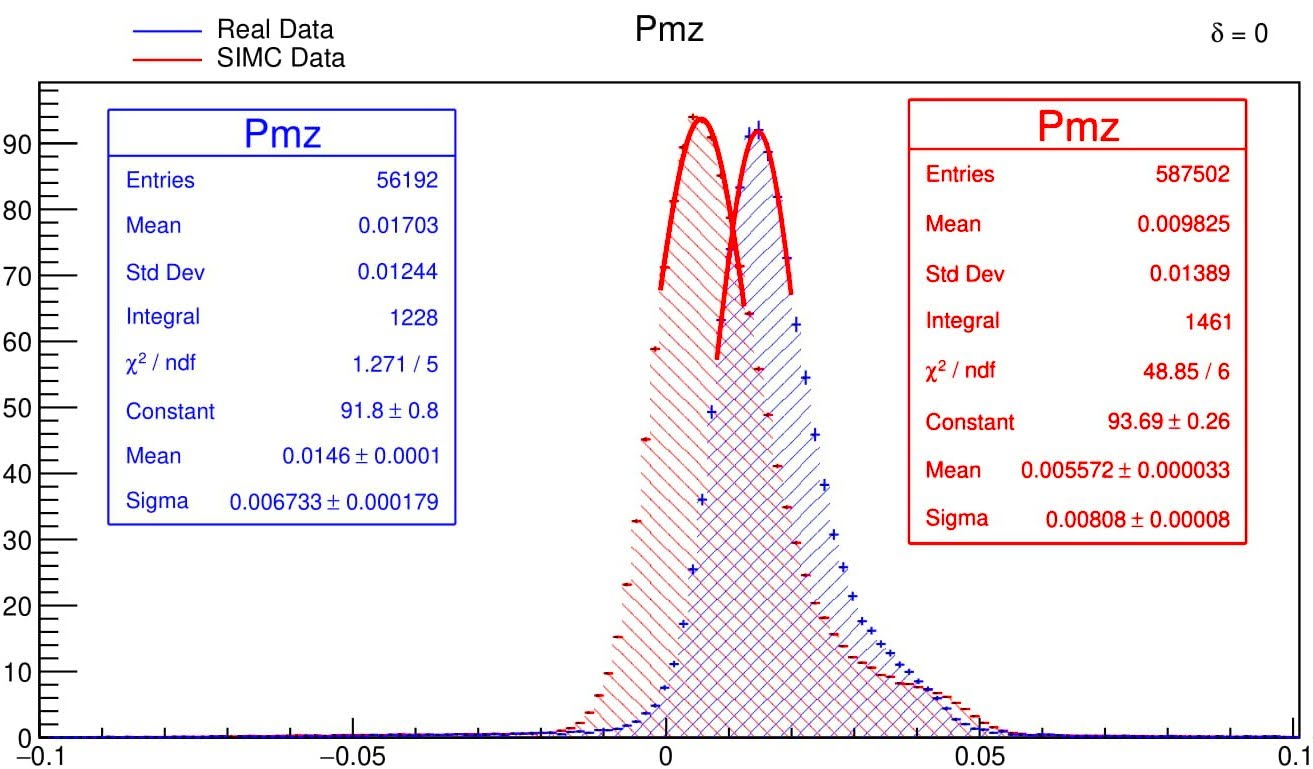
\includegraphics[width=\linewidth]{calibrated data/model 3/Pmz_0.jpg}
  \end{minipage}
\vspace{-.75cm}
  \caption{Optimized spectra for $W$, $E_m$, $P_{mx}$, $P_{my}$, and $P_{mz}$ using Model 3 offsets on a $\delta=0$ run.}
\end{figure}
\vspace{-.75cm}
Model 0 best minimized the distance between the peaks of the SIMC and data histograms compared to all other models. Other models exhibited larger shifts between the peaks of the two lines in nearly all kinematic variables, as seen in Figure 6.

\end{block}
\vspace{-.5cm}
  \begin{exampleblock}{Conclusions}

    \begin{itemize}
        \item Chi-squared minimization is an effective method for kinematic optimization in hydrogen elastic scattering experiments.
        \item Optimization algorithms implemented in Python yielded an effective and modular solution for rapid computation.
        \item Model 0 offers the best agreement between data and SIMC, where deltaP was applied to the final proton momentum before kinematic optimization.
        \item Applying spectrometer offsets to both SIMC and data reconstructions complicates kinematic optimization, though it is necessary to ensure consistent physics event conditions.
    \end{itemize}

  \end{exampleblock}
\vspace{-1cm}
\begin{block}{Future Work}
\begin{itemize}
    \item Apply kinematic optimization over a larger number and range of $\delta$ runs.
    \item Investigate new models that utilize different spectrometer offset variables.
    \item Include out-of-plane offsets with Model 0 for further alignment of $E_m, P_{my},\text{ and } P_{mz}$.
    \item Study the extent to which different proton final momentum correction methods, such as deltaP, affect kinematic optimization.
\end{itemize}
\end{block}
\vspace{-1.25cm}
\begin{block}{References}
\small{
\nocite{yero2020thesis}
\nocite{ibrahim2006thesis}
\printbibliography}
\end{block}


\vspace{-1.25cm}
  \begin{block}{Acknowledgements}
\small We would like to thank The Catholic University of America for the use of their facilities and the Thomas Jefferson National Accelerator Facility for the contribution of their computational resources. We are also grateful to the National Science Foundation for the funding of this project under Award No. 2349155. 

  \end{block}

\end{column}

\separatorcolumn
\end{columns}
\end{frame}

\end{document}